
\documentclass[border=10pt, 12pt]{standalone}
\usepackage[svgnames]{xcolor}
\usepackage{amsmath}
\usepackage{pgfplots}
\pgfplotsset{compat=newest}
\usepackage[sfdefault]{FiraSans}
\usepackage{FiraMono}
\renewcommand*\familydefault{\sfdefault}
\begin{document}
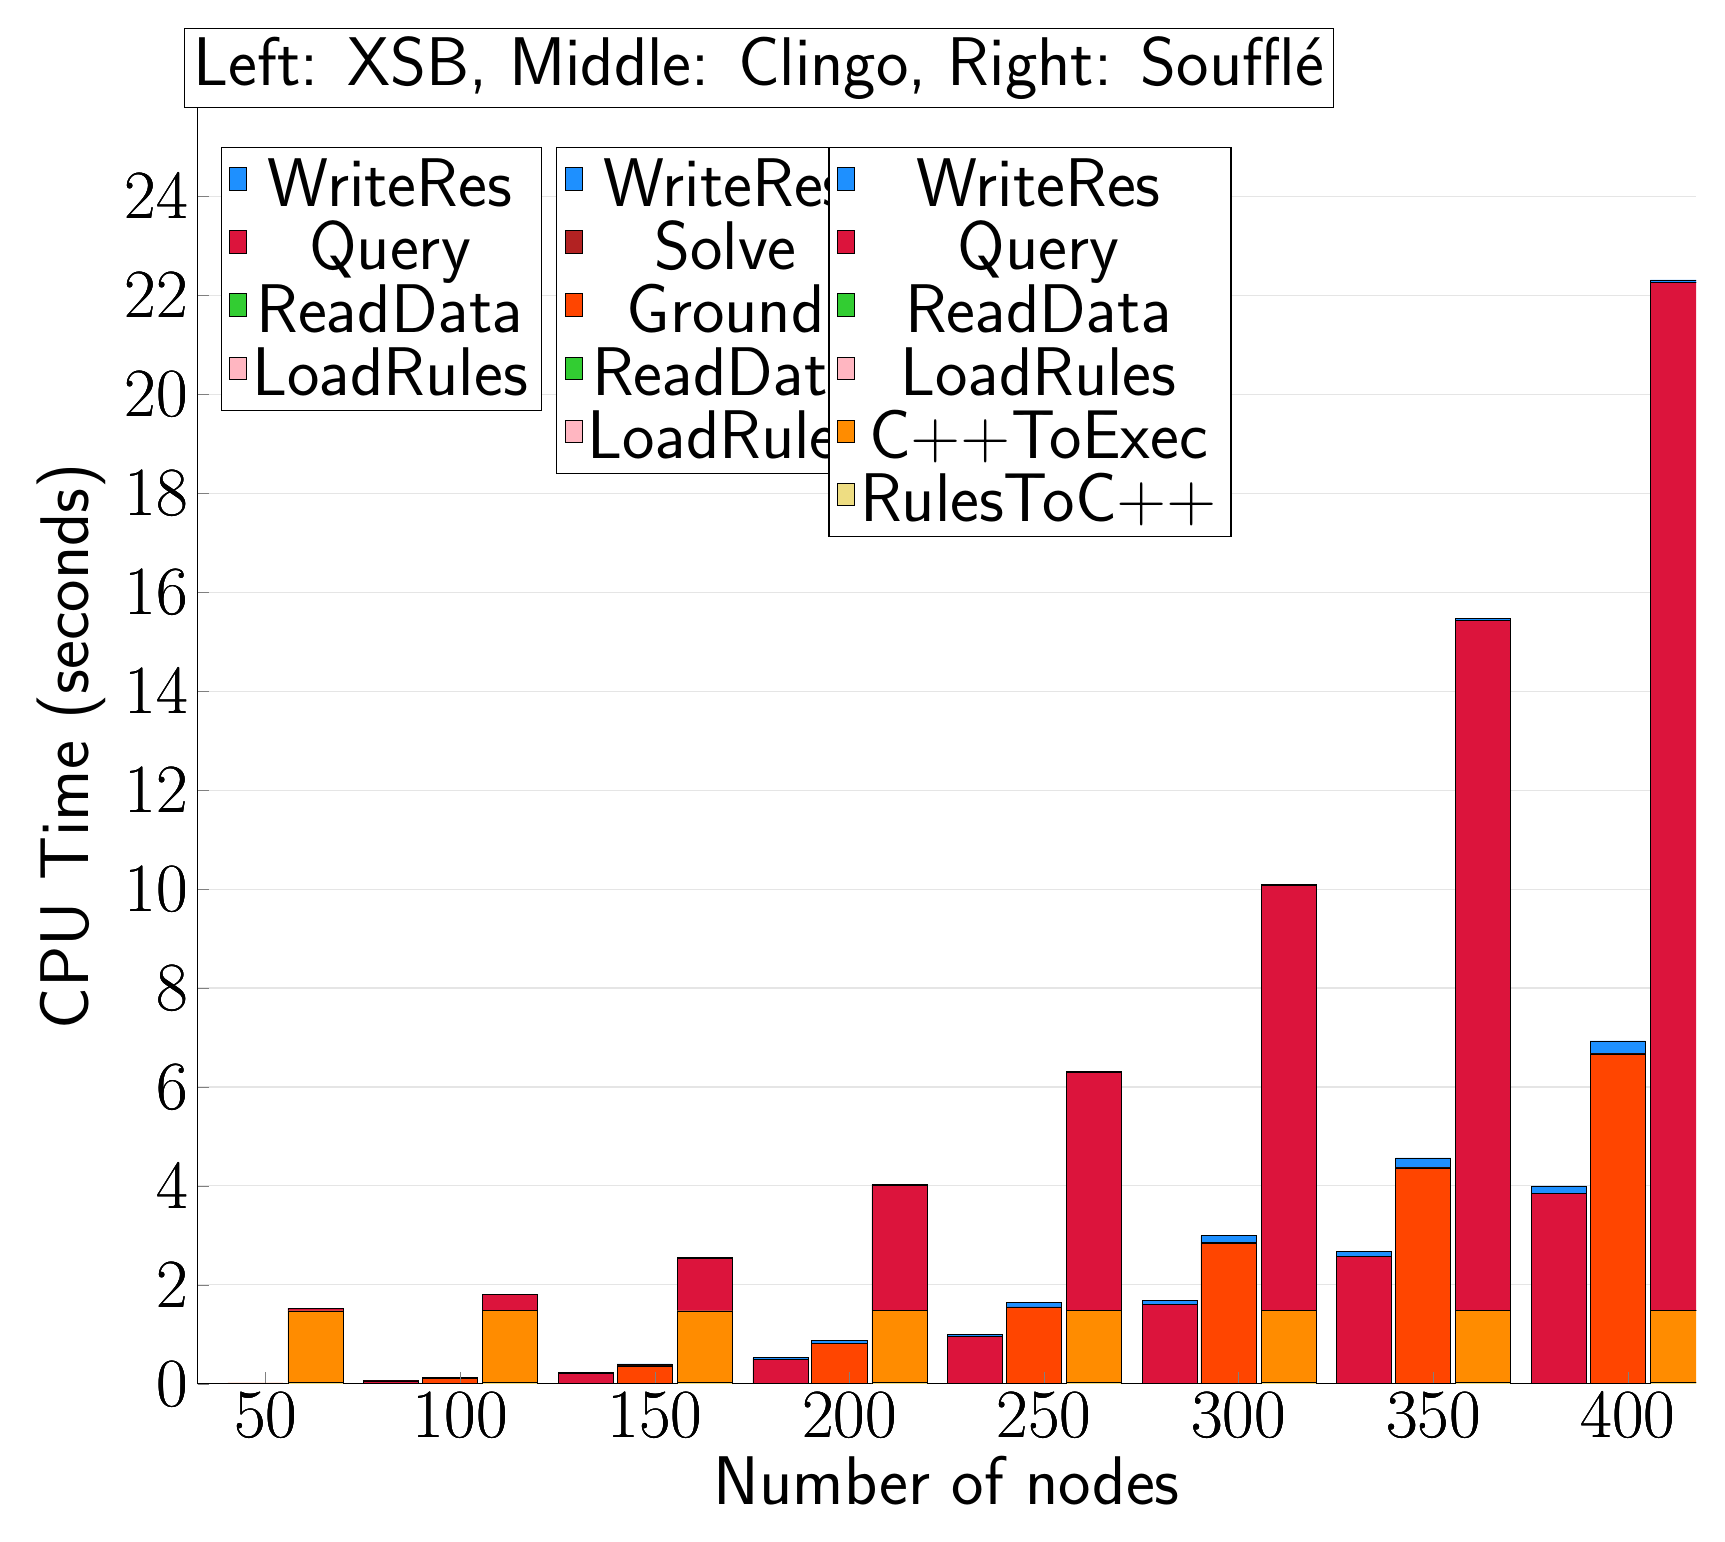
\begin{tikzpicture}
	\begin{axis}[bar shift=-25pt,
			ybar stacked,
			width=1.7\textwidth,
			bar width=0.7cm,
			ymajorgrids, tick align=inside,
			major grid style={draw=gray!20},
			xtick=data,
			ymin=0, ymax=25.779619999999998,
			axis x line*=bottom,
			axis y line*=left,
			enlarge x limits=0.05,
			legend style={
					at={(0.23, 0.97)},
					anchor=north east,
					legend columns=1,
					font=\Huge,
				},
			ylabel={CPU Time (seconds)},
			xlabel={Number of nodes},
			label style={font=\Huge},
			tick label style={font=\Huge},
		]
		\addlegendimage{fill=DodgerBlue, draw=black, line width=0.2pt}
		\addlegendentry{WriteRes}
		\addlegendimage{fill=Crimson, draw=black, line width=0.2pt}
		\addlegendentry{Query}
		\addlegendimage{fill=LimeGreen, draw=black, line width=0.2pt}
		\addlegendentry{ReadData}
		\addlegendimage{fill=LightPink, draw=black, line width=0.2pt}
		\addlegendentry{LoadRules}
		\addplot +[fill=LightPink, draw=black, line width=0.2pt] coordinates {
				(50, 0.0006127000000000001)
				(100, 0.0005970000000000003)
				(150, 0.0006277999999999998)
				(200, 0.0006027000000000001)
				(250, 0.0006254000000000001)
				(300, 0.0006182000000000002)
				(350, 0.0006183999999999996)
				(400, 0.0006082000000000003)
			};
		\addplot +[fill=LimeGreen, draw=black, line width=0.2pt] coordinates {
				(50, 0.00017659999999999958)
				(100, 0.0002153999999999995)
				(150, 0.0002685999999999998)
				(200, 0.0003018999999999996)
				(250, 0.0003526999999999997)
				(300, 0.00040639999999999947)
				(350, 0.0004432000000000007)
				(400, 0.0004793999999999995)
			};
		\addplot +[fill=Crimson, draw=black, line width=0.2pt] coordinates {
				(50, 0.007602300000000001)
				(100, 0.06051260000000001)
				(150, 0.2072289)
				(200, 0.48774570000000006)
				(250, 0.9499592)
				(300, 1.6064833)
				(350, 2.5673429000000003)
				(400, 3.8520795)
			};
		\addplot +[fill=DodgerBlue, draw=black, line width=0.2pt] coordinates {
				(50, 0.0023033999999999997)
				(100, 0.0092248)
				(150, 0.021591100000000005)
				(200, 0.03815340000000001)
				(250, 0.051117000000000024)
				(300, 0.07741620000000005)
				(350, 0.11364100000000006)
				(400, 0.1485033000000001)
			};
	\end{axis}

	\begin{axis}[bar shift=-3.7pt,
			ybar stacked,
			width=1.7\textwidth,
			bar width=0.7cm,
			ymajorgrids, tick align=inside,
			major grid style={draw=none},
			xtick=data,
			ymin=0, ymax=25.779619999999998,
			axis x line*=none,
			axis y line*=none,
			enlarge x limits=0.05,
			legend style={
					at={(0.454, 0.97)},
					anchor=north east,
					legend columns=1,
					font=\Huge,
				},
			label style={font=\Huge},
			tick label style={font=\Huge},
		]
		\addlegendimage{fill=DodgerBlue, draw=black, line width=0.2pt}
		\addlegendentry{WriteRes}
		\addlegendimage{fill=FireBrick, draw=black, line width=0.2pt}
		\addlegendentry{Solve}
		\addlegendimage{fill=OrangeRed, draw=black, line width=0.2pt}
		\addlegendentry{Ground}
		\addlegendimage{fill=LimeGreen, draw=black, line width=0.2pt}
		\addlegendentry{ReadData}
		\addlegendimage{fill=LightPink, draw=black, line width=0.2pt}
		\addlegendentry{LoadRules}
		\addplot +[fill=LightPink, draw=black, line width=0.2pt] coordinates {
				(50, 0.0)
				(100, 0.0)
				(150, 0.0)
				(200, 0.0)
				(250, 0.0)
				(300, 0.0)
				(350, 0.0)
				(400, 0.0)
			};
		\addplot +[fill=LimeGreen, draw=black, line width=0.2pt] coordinates {
				(50, 0.0)
				(100, 0.0)
				(150, 0.0)
				(200, 0.0)
				(250, 0.0)
				(300, 0.0)
				(350, 0.0)
				(400, 0.0)
			};
		\addplot +[fill=OrangeRed, draw=black, line width=0.2pt] coordinates {
				(50, 0.019999999999999997)
				(100, 0.11000000000000001)
				(150, 0.36399999999999993)
				(200, 0.8109999999999997)
				(250, 1.5500000000000003)
				(300, 2.8449999999999998)
				(350, 4.3660000000000005)
				(400, 6.67)
			};
		\addplot +[fill=FireBrick, draw=black, line width=0.2pt] coordinates {
				(50, 0.0)
				(100, 0.0)
				(150, 0.0010000000000000009)
				(200, 0.0050000000000000044)
				(250, 0.006999999999999984)
				(300, 0.010000000000000009)
				(350, 0.011000000000000055)
				(400, 0.015000000000000036)
			};
		\addplot +[fill=DodgerBlue, draw=black, line width=0.2pt] coordinates {
				(50, 0.0)
				(100, 0.01999999999999999)
				(150, 0.03599999999999998)
				(200, 0.05900000000000005)
				(250, 0.09399999999999997)
				(300, 0.14)
				(350, 0.18900000000000003)
				(400, 0.24600000000000008)
			};
	\end{axis}

	\begin{axis}[bar shift=18pt,
			ybar stacked,
			width=1.7\textwidth,
			bar width=0.7cm,
			ymajorgrids, tick align=inside,
			major grid style={draw=none},
			xtick=data,
			ymin=0, ymax=25.779619999999998,
			axis x line*=none,
			axis y line*=none,
			enlarge x limits=0.05,
			legend style={
					at={(0.69, 0.97)},
					anchor=north east,
					legend columns=1,
					font=\Huge,
				},
			label style={font=\Huge},
			tick label style={font=\Huge},
		]
		\addlegendimage{fill=DodgerBlue, draw=black, line width=0.2pt}
		\addlegendentry{WriteRes}
		\addlegendimage{fill=Crimson, draw=black, line width=0.2pt}
		\addlegendentry{Query}
		\addlegendimage{fill=LimeGreen, draw=black, line width=0.2pt}
		\addlegendentry{ReadData}
		\addlegendimage{fill=LightPink, draw=black, line width=0.2pt}
		\addlegendentry{LoadRules}
		\addlegendimage{fill=DarkOrange, draw=black, line width=0.2pt}
		\addlegendentry{C++ToExec}
		\addlegendimage{fill=LightGoldenrod, draw=black, line width=0.2pt}
		\addlegendentry{RulesToC++}
		\addplot +[fill=LightGoldenrod, draw=black, line width=0.2pt] coordinates {
				(50, 0.030000000000000006)
				(100, 0.030000000000000006)
				(150, 0.030000000000000006)
				(200, 0.030000000000000006)
				(250, 0.030000000000000006)
				(300, 0.030000000000000006)
				(350, 0.030000000000000006)
				(400, 0.030000000000000006)
			};
		\addplot +[fill=DarkOrange, draw=black, line width=0.2pt] coordinates {
				(50, 1.4439999999999997)
				(100, 1.4469999999999996)
				(150, 1.4449999999999998)
				(200, 1.4550000000000003)
				(250, 1.4499999999999997)
				(300, 1.457)
				(350, 1.4600000000000002)
				(400, 1.4580000000000002)
			};
		\addplot +[fill=LightPink, draw=black, line width=0.2pt] coordinates {
				(50, 0.0001075)
				(100, 0.00011080000000000001)
				(150, 8.6e-05)
				(200, 9.94e-05)
				(250, 0.00012030000000000001)
				(300, 9.63e-05)
				(350, 0.00011220000000000002)
				(400, 0.00011099999999999999)
			};
		\addplot +[fill=LimeGreen, draw=black, line width=0.2pt] coordinates {
				(50, 0.0003652)
				(100, 0.00045390000000000003)
				(150, 0.0005567999999999999)
				(200, 0.0006571999999999999)
				(250, 0.0007957999999999999)
				(300, 0.0007892000000000001)
				(350, 0.0008537)
				(400, 0.0009533)
			};
		\addplot +[fill=Crimson, draw=black, line width=0.2pt] coordinates {
				(50, 0.0526721)
				(100, 0.3230982)
				(150, 1.066175)
				(200, 2.532561)
				(250, 4.815493)
				(300, 8.581636)
				(350, 13.94141)
				(400, 20.779619999999998)
			};
		\addplot +[fill=DodgerBlue, draw=black, line width=0.2pt] coordinates {
				(50, 0.0009512000000000001)
				(100, 0.0030570000000000003)
				(150, 0.0064953)
				(200, 0.0115408)
				(250, 0.0179507)
				(300, 0.0255558)
				(350, 0.0347213)
				(400, 0.044857400000000006)
			};
	\end{axis}


	\node[anchor=south, draw, fill=white] at (rel axis cs:0.42,1) {\Huge Left: XSB, Middle: Clingo, Right: Soufflé};
\end{tikzpicture}
\end{document}
